\chapter{DESAIN DAN PERANCANGAN}
  Pada bab ini dibahas mengenai analisis dan perancangan dari sistem. 
  \section{Deskripsi Umum Sistem}    
    Sistem yang akan dibuat adalah sebuah sebuah sistem yang dapat membuat sebuah kontainer \textit{docker} secara otomatis untuk setiap satu \textit{client} yang telah \textit{login} ke dalam sistem. Saat \textit{client} belum \textit{login} ke dalam sistem, maka \textit{client} tersebut akan diarahkan ke halaman \textit{login} dari sistem. Saat \textit{client} mencoba untuk \textit{login} ke dalam sistem, maka sistem akan melakukan pengecekan di dalam basis data apakah \textit{username} dan \textit{password} yang di\textit{input}kan sudah benar atau salah. 
    
    Setelah \textit{client} berhasil \textit{login} ke dalam sistem, sistem akan mengirimkan perintah untuk membuat kontainer \textit{docker} yang berisikan \textit{mitmproxy} ke \textit{docker host}. Setelah berhasil membuat kontainer \textit{docker} untuk client tersebut, maka \textit{traffic} internet dari \textit{client} tersebut akan diarahkan ke kontainer \textit{docker} berisikan \textit{mitmproxy} yang baru saja dibuat. Setelah itu akan client baru dapat untuk mengakses internet.
  
  \section{Kasus Penggunaan}
  Terdapat empat aktor dalam sistem yang akan dibuat yaitu \textit{Client}, \textit{Server Login}, \textit{Administrator}, dan \textit{Docker Host}. \textit{Client} adalah aktor yang melakukan proses \textit{login} ke dalam sistem, \textit{server login} adalah aktor yang melakukan proses permintaan penyediaan kontainer \textit{docker}, \textit{administrator} adalah aktor yang melakukan monitoring kontainer \textit{docker} yang sedang berjalan, sedangkan \textit{docker host} adalah aktor yang akan menjadi tempat penyedia kontainer dan menerima perintah penyediaan kontainer. Diagram kasus penggunaan menggambarkan kebutuhan - kebutuhan yang harus dipenuhi sistem. Diagram kasus penggunaan digambarkan pada Gambar \ref{gambarDiagramKasusPenggunaan}.
  \begin{figure}[!h] % h = pasti berada di bawah teks yang ada di atas
  \centering
  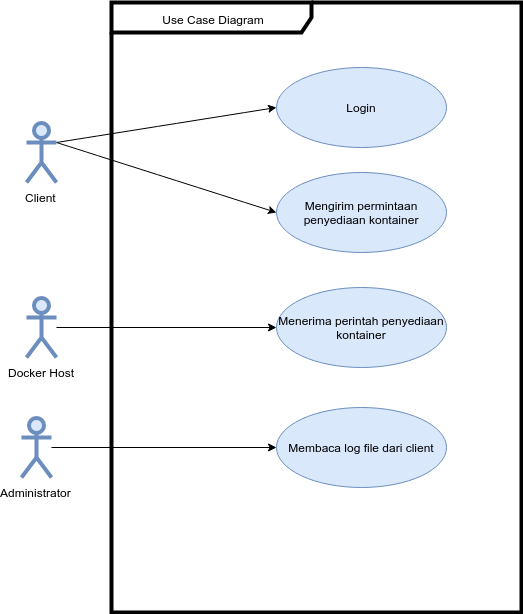
\includegraphics[width=\linewidth]{images/bab3/usecase}
  \caption{Digram Kasus Penggunaan}
  \label{gambarDiagramKasusPenggunaan}
  \end{figure}
  \\
		    		    
	Digram kasus penggunaan pada Gambar \ref{gambarDiagramKasusPenggunaan} dideskripsikan masing-masing pada Tabel \ref{tabelKodeKasusPenggunaan}.
    \begin{longtable}{|p{0.25\textwidth}|p{0.24\textwidth}|p{0.35\textwidth}|} % L = Rata kiri untuk setiap kolom, | = garis batas vertikal.

% Kepala tabel, berulang di setiap halaman
\caption{Daftar Kode Kasus Penggunaan} \label{tabelKodeKasusPenggunaan} \\
\hline
\textbf{Kode Kasus Penggunaan} & \textbf{Nama Kasus Penggunaan} & \textbf{Keterangan} \\ \hline

\endhead
\endfoot
\endlastfoot

% Isi Tabel
UC-0001 & \textit{Login} & \textit{Client} dapat \textit{login} ke dalam sistem. \\ \hline
UC-0002 & Mengirim Permintaan Penyediaan Kontainer \textit{Docker} & \textit{Server login} dapat mengirimkan permintaan penyediaan kontainer \textit{docker} pada \textit{docker host}. \\ \hline
UC-0003 & Menerima Perintah Penyediaan Kontainer \textit{Docker}  &  Proses dimana \textit{docker host} akan menerima perintah dari sistem, untuk menyediakan kontainer secara otomatis.\\ \hline
UC-0004 & Membuat Aturan untuk Mengarahkan \textit{Traffic Client}  &  Proses dimana \textit{docker host} akan membuat aturan untuk mengarahkan \textit{traffic client} ke halaman \textit{login} dari sistem atau untuk membuat aturan untuk mengarahkan \textit{traffic client} ke kontainer \textit{docker} dari tiap-tiap \textit{client}. \\ \hline
UC-0005 & Membaca \textit{Log File} dari \textit{Client}  &  Proses dimana \textit{administrator} dari sebuah jaringan dapat membaca \textit{log file} dari client secara \textit{live} ataupun juga ketika \textit{client} telah selesai menggunakannya.\\ \hline
\end{longtable}

  \section{Arsitektur Sistem}
  	Pada Sub-bab ini, dibahas mengenai tahap analisis arsitektur, analisis teknologi dan desain sistem yang akan dibangun.
    \subsection{Desain Umum Sistem}
      \indent Berdasarkan deskripsi umum sistem yang telah ditulis diatas, dapat diperoleh kebutuhan sistem ini, diantaranya :
        \begin{enumerate}
        \item Pemeriksaan data kontainer yang sudah dibuat pada \textit{docker host}.
        \item Pembuatan aturan untuk mengarahkan \textit{traffic client} ke halaman \textit{login} dari sistem.
        \item Pembuatan aturan untuk mengarhakn \textit{traffic client} ke kontainer \textit{docker} dari tiap-tiap \textit{client}.
        \item Pemasangan kontainer pada \textit{docker host}.
        \item Pembacaan \textit{log file} dari \textit{client}.
        \end{enumerate} 
      
      \indent Untuk memenuhi kebutuhan sistem tersebut, penulis membagi sistem menjadi beberapa komponen. Komponen yang akan dibangun antara lain: 
      \begin{enumerate} 
	  \item Pemeriksaan data kontainer yang sudah dibuat pada \textit{docker host}.\\
		  Berfungsi agar sistem mengetahui apakah \textit{client} dengan IP tersebut diperbolehkan mengakses internet atau tidak.
	  \item Pembuatan aturan untuk mengarahkan \textit{traffic client} ke halaman \textit{login} dari sistem.\\
		  Berfungsi untuk mengarahkan tiap \textit{client} yang belum \textit{login} ke dalam sistem ke halaman \textit{login} dari sistem. Hal ini dilakukan dengan menjalankan sebuah \textit{script} dengan menggunakan \textit{iptables} pada \textit{docker host}.
	  \item Pembuatan aturan untuk mengarahkan \textit{traffic client} ke kontainer \textit{docker} dari tiap-tiap \textit{client}.\\
		  Berfungsi untuk mengarahkan tiap \textit{client} yang telah berhasil \textit{login} ke kontainer \textit{docker} dari tiap-tiap \textit{client}. Hal ini dilakukan dengan menjalankan sebuah \textit{script} dengan menggunakan \textit{iptables} pada \textit{docker host}.
	  \item Pemasangan kontainer pada \textit{docker host}.\\
		  Berfungsi untuk memasangkan kontainer \textit{docker} pada \textit{docker host} secara otomatis. Hal ini dilakukan dengan menjalankan sebuah perintah penyediaan kontainer pada \textit{docker host}.
	  \item Pembacaan \textit{log file} dari \textit{client}.
		  Berfungsi untuk melihat apa saja yang telak diakses oleh \textit{client}. \textit{Log} yang tersimpan terdapat \textit{log} HTTP maupun \textit{log} HTTPS. Hal ini dilakukan dengan menjalankan sebuah perintah untuk melihat \textit{log file} dari suatu \textit{client}.
        
      \end{enumerate}
      \indent Pada pada Gambar \ref{Arsitektur Komponen Sistem} ditunjukkan arsitektur sistem secara umum dengan detail-detail dari kompenen yang terdapat didalamnya. Setiap komponen tersebut akan diimplementasikan dengan teknologi pendukung yang dibutuhkan.\\
      
      \begin{figure}[H]
        \centering
        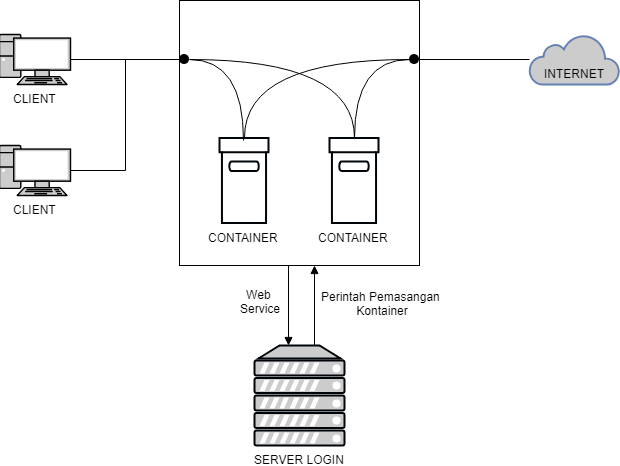
\includegraphics[width=\linewidth]{images/bab3/arsitekttur_komponen}
        \caption{Arsitektur Komponen Sistem}
        \label{Arsitektur Komponen Sistem}
      \end{figure} 
    \subsection{Perancangan Pemeriksaan Data Kontainer yang Sudah Dibuat pada \textit{docker host}.}
    Pemeriksaan data kontainer yang sudah dibuat pada \textit{docker host} adalah komponen yang bertugas untuk melakukan pemeriksaan pada setiap kontainer \textit{docker} pada \textit{docker host} yang sudah dibuat. Jika pada saat dilakukan pemeriksaan ternyata belum dibuatkan kontainer \textit{docker} pada \textit{docker host}, maka \textit{client} akan diarahkan menuju ke halaman \textit{login} sistem. Setelah \textit{} tersebut berhasil login, maka sistem akan membuat secara otomatis kontainer \textit{docker} pada \textit{docker host}. Jika pada saat dilakukan pemeriksaan ternyata sudah dibuatkan kontainer \textit{docker} pada \textit{docker host}, maka \textit{client} tersebut akan dibuatkan sebuah \textit{rules} menggunakan iptables yang berfungsi untuk mengijinkan \textit{client} tersebut mengakses internet.
    
    Dikarenakan ada beberapa kebutuhan yang harus dipenuhi, komponen pada pemeriksaan data kontainer \textit{docker} yang sudah dibuat pada \textit{docker host} dibagi lagi menadji 2 sub komponen, yaitu:
   	\begin{enumerate}
   		\item Basis Data \\
   		Basis data berfungsi sebagai tempat penyimpanan data \textit{username} dan \textit{password} yang digunakan untuk \textit{login} ke dalam sistem. Basis data juga berfungsi sebagai tempat penyimpanan data kontainer \textit{docker} yang sudah dibuat.
   		\item \textit{Web Service} \\
   		\textit{Web service} berfungsi sebagai antarmuka untuk \textit{client} ketika \textit{client} akan \textit{login} ke dalam sistem. Selain itu \textit{web service} juga berfungsi sebagai penerima permintaan dari \textit{client}, yang nantinya akan membuat sebuah kontainer \textit{docker} secara otomatis pada \textit{docker host}.
   	\end{enumerate}
   	
   	Pada tugas akhir ini, bahasa Python dipilih sebagai bahasa pemrograman yang digunakan untuk mengimplementasikannya. Lalu, pada bagian penyimpanan data atau basis data, MySQL dipilih sebagai RDBMS untuk tugas akhir ini.
   	\subsubsection{Desain Basis Data}
   	Komponen basis data berfungsi sebagai tempat penyimpanan data \textit{username} dan \textit{password} yang digunakan untuk \textit{login} ke dalam sistem. Dalam basis data ini terdapat satu entitas dan dua atribut, ditunjukkan pada Tabel \ref{atributdb}
   	\begin{ltabulary}{|L|L|} 
   		\caption{Atribut basis data NRP mahasiswa} \label{atributdb} \\
   		\hline
   		\textbf{Nama} & \textbf{Tujuan} \\ \hline
   		\endhead
   		\endfoot
   		\endlastfoot
   		% Isi Tabel
   		\textbf{ID} & ID \textit{server}\\ \hline
   		\textbf{Name} & Hostname \textit{server} \\ \hline
   		%         \textbf{Status} & Status sensor(aktif/tidak aktif) \\ \hline
   	\end{ltabulary}
   	
   	Selain itu, komponen basis data juga berfungsi sebagai tempat penyimpanan data kontainer \textit{docker} yang sudah dibuat. Dalam basis data ini terdapat satu entitas dan tiga atribut, ditunjukan pada Tabel \ref{atributdb}
   	\begin{ltabulary}{|L|L|} 
   		\caption{Atribut basis data kontainer} \label{atributdb} \\
   		\hline
   		\textbf{Nama} & \textbf{Tujuan} \\ \hline
   		\endhead
   		\endfoot
   		\endlastfoot
   		% Isi Tabel
   		\textbf{ID} & ID \textit{server}\\ \hline
   		\textbf{Name} & Hostname \textit{server} \\ \hline
   		%         \textbf{Status} & Status sensor(aktif/tidak aktif) \\ \hline
   	\end{ltabulary}
	   
   	\subsubsection{Desain Web Service}
	Komponen web service berfungsi untuk menyediakan antarmuka halaman \textit{login} untuk \textit{client} dan untuk menerima permintaan pembuatan kontainer \textit{docker} secara otomatis pada \textit{docker host} setelah terdapat \textit{client} yang berhasil \textit{login} ke dalam sistem.
	
	\subsection{Pembuatan Aturan untuk Mengarahkan \textit{Traffic Client} ke Halaman \textit{Login} dari Sistem}
	asd
	
	\subsection{Pembuatan Aturan untuk Mengarahkan \textit{Traffic Client} ke Kontainer \textit{Docker} dari Tiap-Tiap \textit{Client}}
	asd
   	
    \subsection{Perancangan Pemasangan Kontainer pada \textit{Docker Host}}
	Pemasangan kontainer adalah kompenen yang berfungsi untuk memasangkan kontainer \textit{docker} yang berisikan \textit{mitmproxy} pada \textit{docker host} setelah ada permintaan dari \textit{client} yang telah berhasil \textit{login} ke dalam sistem. Proses ini dilakukan secara otomatis, dan nama dari kontainer \textit{docker} tersebut akan sesuai dengan IP dari \textit{client} yang telah berhasil \textit{login} ke dalam sistem.   

      